\documentclass[9pt,conference,a4paper]{IEEEtran}
\IEEEoverridecommandlockouts

%\usepackage{...}

\usepackage{graphicx}
\usepackage{floatrow}

\title{Constrained spherical deconvolution on signal and ODF values.}
\author{
	\IEEEauthorblockN{
		Eleftherios Garyfallidis\IEEEauthorrefmark{1},
		Samuel St-Jean\IEEEauthorrefmark{1},
		Michael Paquette\IEEEauthorrefmark{1},
		Pierrick Coup\'e\IEEEauthorrefmark{2},
		Maxime Descoteaux\IEEEauthorrefmark{1}
	}

	\IEEEauthorblockA{\IEEEauthorrefmark{1} Sherbrooke Connectivity Imaging Lab (SCIL), Computer Science department, Universit\'e de Sherbrooke, Sherbrooke, Canada}
	\IEEEauthorblockA{\IEEEauthorrefmark{2} CNRS, Laboratoire Bordelais de Recherche en Informatique, Bordeaux, France}
}

\begin{document}
\maketitle

For the purpose of the ISBI HARDI reconstruction challenge 2013 and for the categories DTI and HARDI we reconstructed the diffusion datasets using two well established methods: a) Spherical Deconvolution Transform (SDT) \cite{descoteaux-deriche-etal:09}, \cite{Descoteaux2008} and b) Constrained Spherical Deconvolution (CSD) \cite{tournier-calamante-etal:07}.

The SDT is a sharpening operation which transforms the smooth diffusion ODF into a sharper fiber ODF. The method is inspired by CSD \cite{tournier-calamante-etal:07} with the main difference that the CSD is applied directly to the initial signal and the SDT directly to the ODFs. 

The idea here is that an ODF for example the analytical Q-ball ODF $\psi_{QBI}$ can be formed by convolution between the single fiber diffusion ODF kernel, $R$ and the true fiber ODF $\psi_{SDT}$. 
\begin{equation}
\psi_{QBI}(\mathbf{u})=\displaystyle\int_{|w|=1} R(\mathbf{u} \cdot \mathbf{w}) \psi_{SDT}(\mathbf{w}) dw\label{eq:Conv}
\end{equation}
Therefore, the deconvolution of $\psi_{QBI}$ can recover a sharper $\psi_{SDT}$. We can derive the formulat for the $\psi_{SDT}$ using symmetrized spherical harmonics.
\begin{equation}
\psi_{SDT}(\mathbf{u})=\displaystyle\sum_{j=1}^{R}2\pi P_{l_{j}}(0) \frac{c_j}{f_j}Y_{j}(\mathbf{u})\label{eq:ODF_SDT}
\end{equation}
For the derivation of the formula see \cite{descoteaux-deriche-etal:09}.

The deconvolution is a fast converging iterative process. The main choice to be considered both for SDT and CSD is the estimation of the single fiber response function $R$. We assume that $R$ is derived from a prolate tensor. The eigenvalues of this tensor are estimated from the voxels with FA $> 0.7$.

In order to deal with the high levels of noise, the diffusion weighted (DW) datasets for SNR 10 and 20 were denoised with the adaptive nonlocal means \cite{manjon-coupe:10} using a rician noise model. As proposed in \cite{descoteaux-wiest-daessle-etal:08}, each DW images were processed independently. The DW dataset with SNR 30 was left intact and no further denoising was performed.

\begin{figure}[h]
\begin{centering}
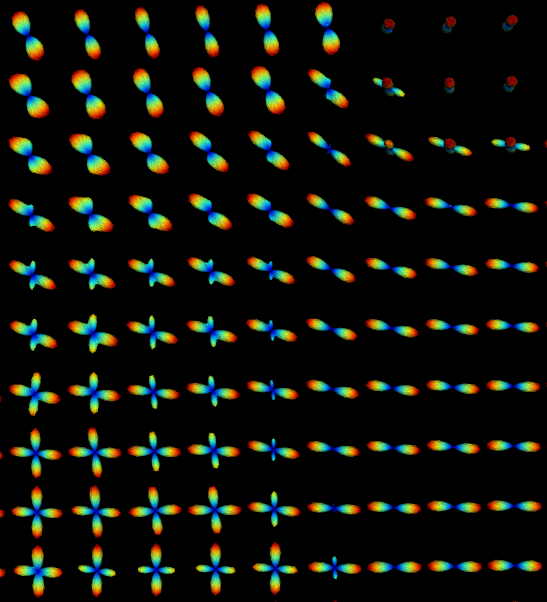
\includegraphics{csd_test_snr10}
\end{centering}
\caption{A detail of our CSD-based reconstruction ODFs with the denoised test data set (SNR 10) provided by the organizers of the HARDI reconstruction challenge 2013}
\end{figure}

\begin{figure}[h]
\begin{centering}
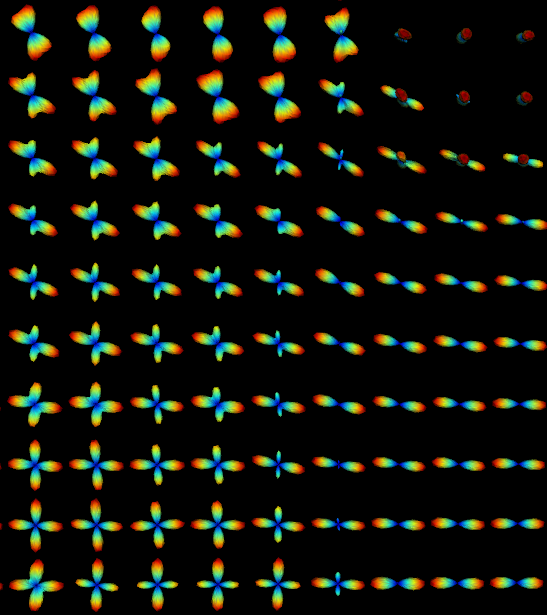
\includegraphics{sdt_test_snr10}
\end{centering}
\caption{A detail of our SDT-based reconstruction ODFs with the denoised test data set (SNR 10) provided by the organizers of the HARDI reconstruction challenge 2013}
\end{figure}



The code for these methods is available in dipy.org.

...

...

...

...

...

...

\bibliographystyle{ieeetr}
\bibliography{/home/eleftherios/Documents/scil-bibtex/scilBibTex}

\end{document}


